%!TEX root = ../main.tex
\catalin{Messages ID or Nodes ID?? How different are they and why should we choose one over the other?}
\subsection{CAN Bus Tests}
With the CAN controller available on the PS of the Zybo, the CAN bus will be tested to determine the transmission abilities of the network.
The transceivers are able to work at up to 8 Mb/s, while the CAN controllers on the Zybo only guarantee functionality up to 1 Mb/s. 
As the final implementation should be done in PL, there is nothing preventing the controller working at 8 Mb/s -- the FPGA can easily produce and interpret signals up to or beyond 8 Mb/s.

\paragraph{Latency tests:} The time it takes to send one large frame
 

\paragraph{Bandwidth:} How much raw data can be transmitted per unit time

%\paragraph{Message filtering}
%Three Zybos will be needed for this test.
%One will act as a transmitter, and the two others will receive messages.\\
%The transmitting node will shift back and forth between three message IDs, and write a recursive message, i.e. counting up from zero.
%One receiving node will only accept one message ID, the other node will only accept another message ID, and the third message ID will be ignored by both.


\paragraph{Priority when multiple node sending:} Ensuring, that higher message ID make way for the lower ones 

\subsubsection{Latency Test}\label{sub:CAN_latency}
For this test, only two Zybos are needed.
One node prepares a frame for transmission, then sets a GPIO pin high.
It then performs the necessary checks and writes the message details to the TX fifo, and then sets its GPIO pin low. \\
The other node will then wait for the full message frame to be received, and then set its GPIO pin high.
Once the metadata of the message (data length and message ID) has been intepreted, the voltage goes low again.
Using an oscilloscope, it is possible to measure the time it takes to send a message.\\

The test will be performed for an 8 byte frame.
The messages will be constructed, so that bit stuffing doesn't occur by writing 0xA1 to 0xA8. 
The resulting voltage measurements are displayed on the figure below

\begin{figure}[h]
	\centering
	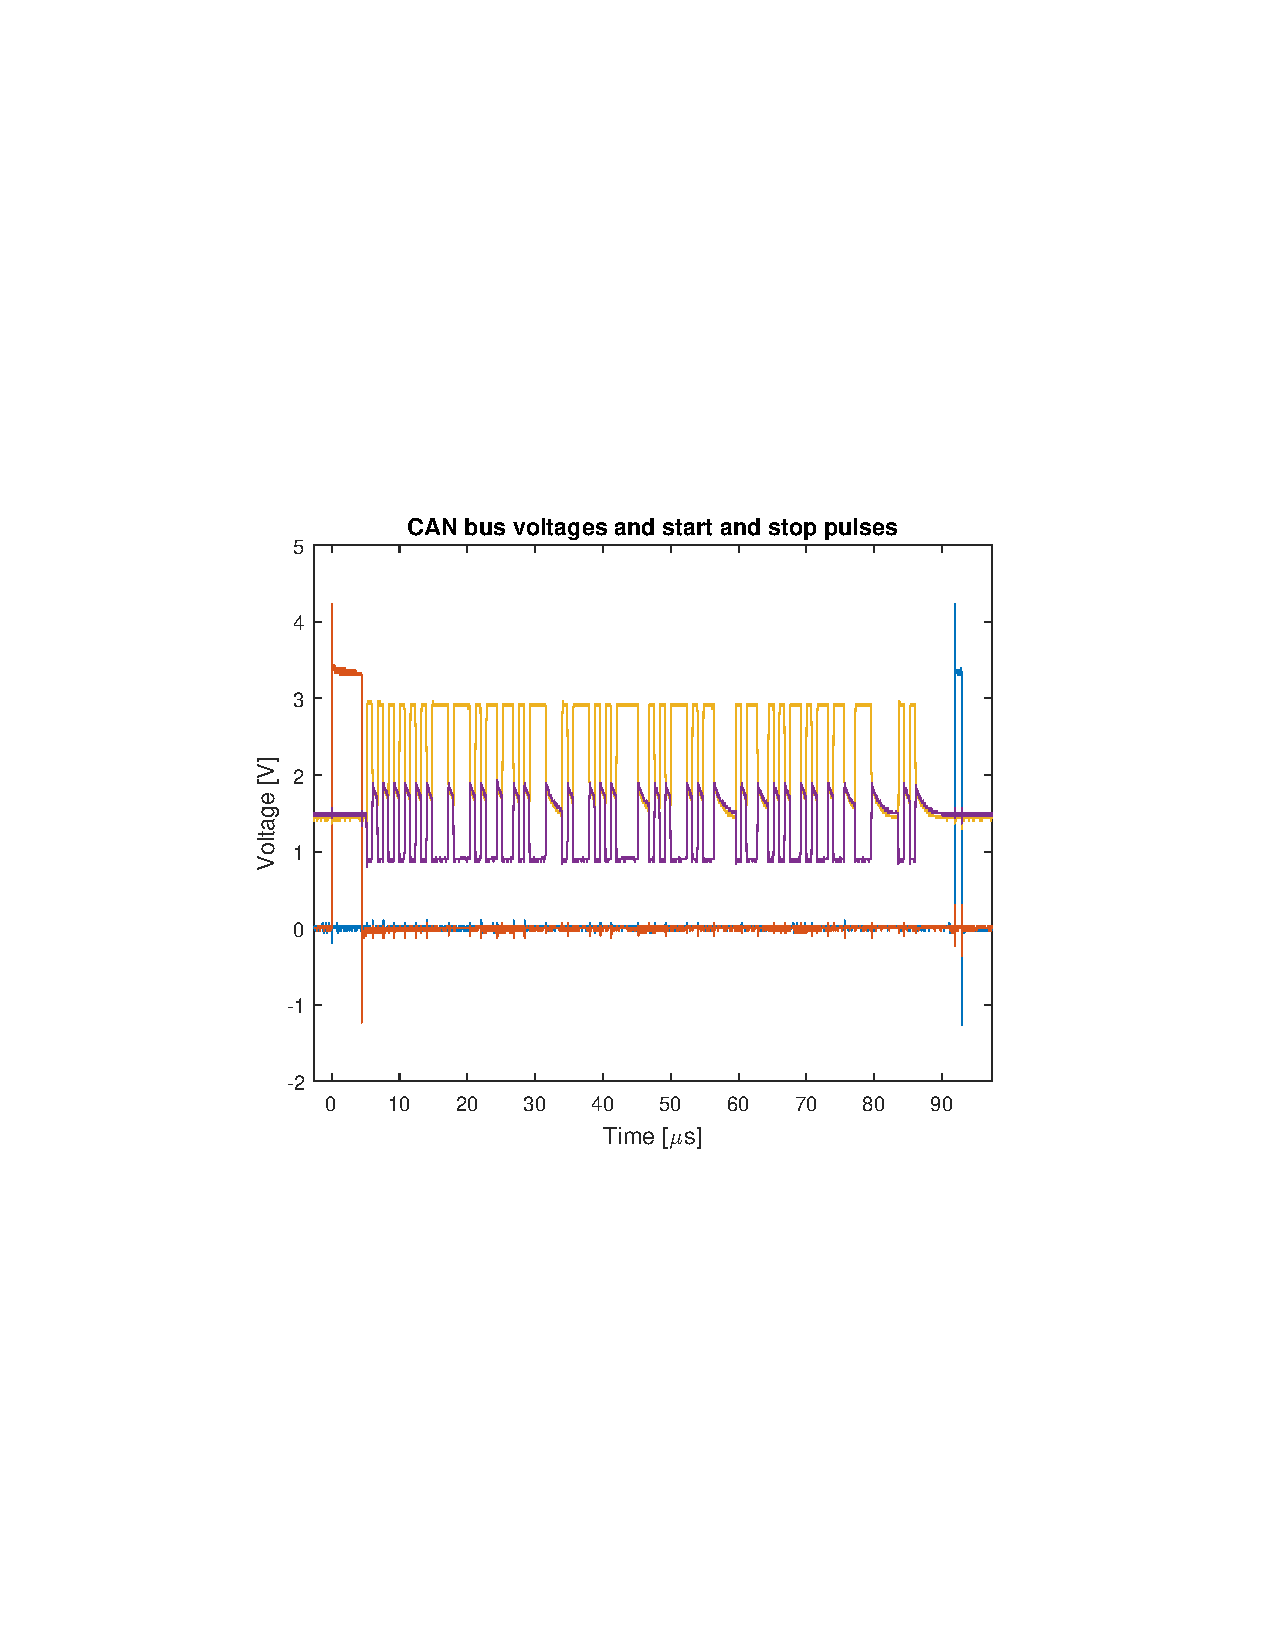
\includegraphics[width = \linewidth]{graphics/CAN_test1_raw}
	\caption{Start and stop pulses for an 8 byte CAN message}
	\label{fig:CAN_test1_raw}
\end{figure}

The time from the red voltage goes low, to the time the blue voltage goes high is $87.5 \si{\micro\second}$.
This is of course very dependent on the particular controller used for this test, which according to the datasheet can work up to 1 MHz.
Measuring this test shows, that pulses come at 1.25 MHz.
The software used for basis of this test does allow to adjust a pre-scaler, so that the controller works faster, but it is not able receive frames at a higher rate than 1.25 MHz.\\

The CAN bus voltage can be interpreted to bits, to show what's actually being transmitted.
This is done by measuring the voltage difference between the yellow and purple graphs, keeping in mind, that a difference in voltage corresponds to a zero, while no difference corresponds to a one.
The CAN frame is displayed and interpreted on the figure below.

\begin{figure}[h]
	\centering
	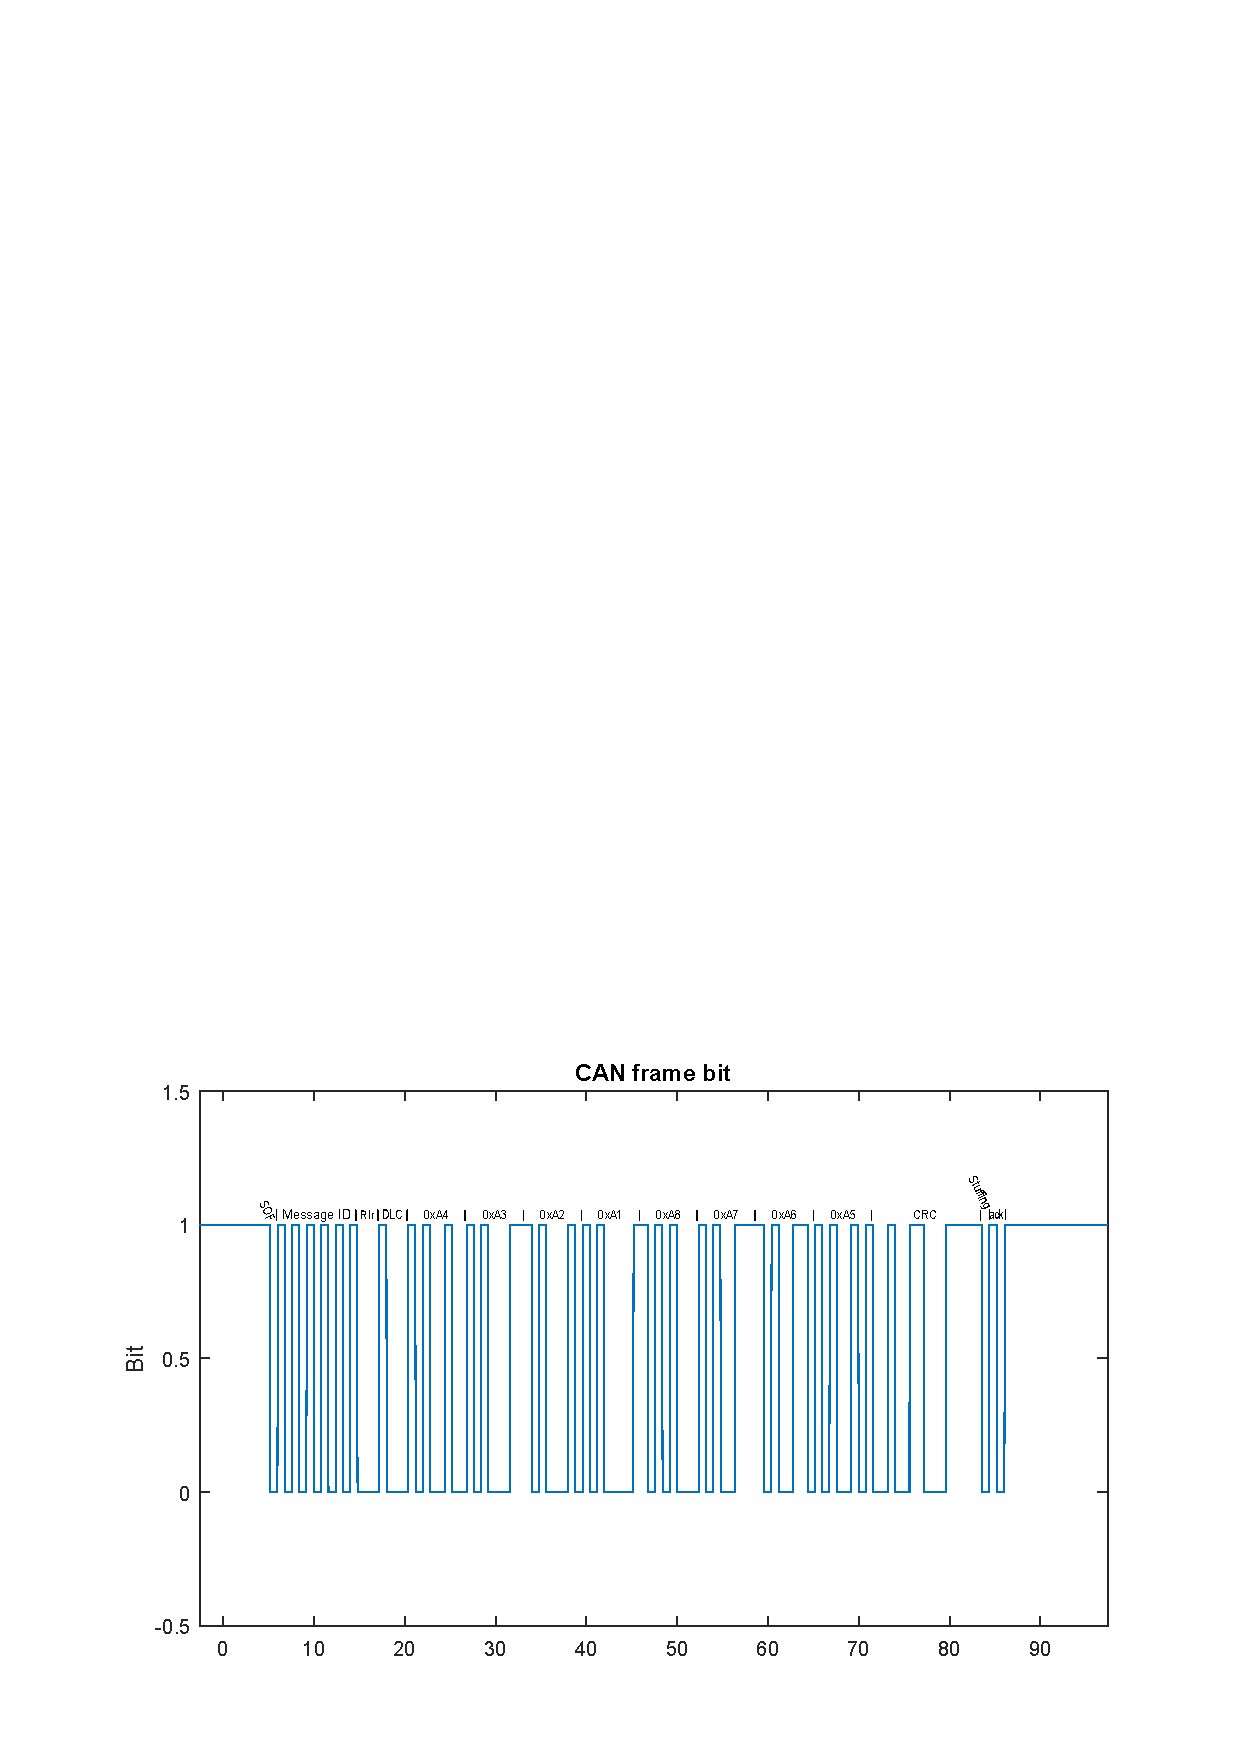
\includegraphics[width = \linewidth]{graphics/CAN_test1_message}
	\caption{Bit interpretation of the CAN frame. RIr  is the tree bits: RTR, ID Extention and r0, which are all 0.}
	\label{fig:CAN_test1_message}
\end{figure}

The data portion of the frame is bitwise big endian, but bytewise little endian. 
The message to be sent was codes as two 32 bit unsigned integers: 0xA1A2A3A4 and 0xA5A6A7A8.
The controller then swapped the bytes around, causing the data to become little endian.
This is a convention implemented by the CAN controller, and as the same endianness is applied when sending and receiving the frame, it doesnt matter -- the CAN bus does not care about the order bits in the data portion. 
The message was received correctly.\\

The CRC was calculated automatically by the controller.
Unfortunately it ends on five consecutive 1's, meaning that a 0 must be stuffed in-between the delimiter, causing the frame to be one bit longer.\\

Additionally this controller uses 5 bits for the IFS part of the frame, rather than the mandatory minimum of 3 bits. 



\subsubsection{Bandwidth}\label{sub:CAN_bandwidth}
This will be calculated, as the faster controllers are not available.
Bandwidth is considering the amount of net data being transmitted per unit time, when excluding the overhead.
Bandwidth will be calculated for 8 byte frames, and bit stuffing will be omitted.\\

The maximum operating data rate for the transceivers is 8 Mb/s.
As mentioned in section~\ref{sub:CanMessageFrame}, the CAN frame 47 bits of overhead. 
Including 8 bytes of data, this comes up to 111 bits. 
Time per frame is:

\begin{equation}
\frac{111}{8 \cdot 10^6} = 1.39 \cdot 10^-5
\end{equation}

As each frame contains 8 bytes of data, the data rate becomes:

\begin{equation}
\frac{8}{1.39 \cdot 10^-5}= 5.77 \cdot 10^5
\end{equation}

That means, that the effective transfer rate is 577 kB/s, or 4.61 Mb/s

\subsubsection{Message Priority}\label{sub:CAN_message priority}
Two Zybos will be needed for this test.
Both Zybos will be prompted to send a message when an interrupt occurs on an input pin. 
The data part of the messages don't matter, but the message IDs do; they need to be different.
Zybo A will send the message ID 0b10101000000.
Zybo B will have the message ID 0b10101010000.
That means, that Zybo A has higher priority, and Zybo B will stop trying to send a message when the seventh bit occurs, and receive instead.
It is assumed, that once Zybo A is done sending, (and its frame is acknowledged), Zybo B will succesfully retry its transmission. 
